\documentclass[a4paper]{article}
\usepackage[margin=3.3cm]{geometry}
\usepackage{amsmath}
\usepackage[x11names]{xcolor}
\usepackage{xspace}
\usepackage{adjustbox}
\usepackage{graphicx}
\usepackage{fontspec}
\setmainfont{STIX Two Text}
\usepackage{unicode-math}
\setmathfont{STIX Two Math}
\usepackage[indent]{parskip}
\usepackage{wrapfig}
% \usepackage[style=numeric,sorting=ynt]{biblatex}
%\addbibresource{quantumstars.bib}
\graphicspath{ {./images/} }
\usepackage[exponent-product=\cdot]{siunitx}
\usepackage{derivative}
\usepackage{caption}
\usepackage{subcaption}
\usepackage{microtype}
\usepackage{listings}
%\usepackage[colorlinks=true,linkcolor=RoyalBlue3,urlcolor=Brown2]{hyperref}
\usepackage[colorlinks=true,linkcolor=blue]{hyperref}
\usepackage{matlab-prettifier}

\DeclareSIUnit\erg{erg}
\DeclareSIUnit\Msunc{\Msun c^2}

\definecolor{codegreen}{rgb}{0,0.6,0}
\definecolor{codegray}{rgb}{0.5,0.5,0.5}
\definecolor{codepurple}{rgb}{0.58,0,0.82}
\definecolor{backcolour}{rgb}{0.95,0.95,0.92}

\lstdefinestyle{mystyle}{
    backgroundcolor=\color{backcolour},   
    commentstyle=\color{codegreen},
    keywordstyle=\color{magenta},
    numberstyle=\tiny\color{codegray},
    stringstyle=\color{codepurple},
    basicstyle=\ttfamily\footnotesize,
    breakatwhitespace=false,         
    breaklines=true,                 
    captionpos=b,                    
    keepspaces=true,                 
    numbers=left,                    
    numbersep=5pt,                  
    showspaces=false,                
    showstringspaces=false,
    showtabs=false,                  
    tabsize=3
}

\lstset{style=mystyle}

\newcommand\elec{\mathrm{e^-}}
\newcommand\numberthis{\addtocounter{equation}{1}\tag{\theequation}}
\newcommand\M{\mathcal{M}}
\newcommand\Mbar{\bar{\mathcal{M}}}
\newcommand\Msun{M_{\odot}}

\DeclareMathOperator{\asinh}{asinh}

\title{Quantum stars}
\author{Group 11\\Pau Blancafort\quad Josep Pérez\quad Eudald Puy\quad Aitor da Rocha}
\date{\today}

\begin{document}

\pagenumbering{gobble}

\maketitle

\begin{center}

\includegraphics[width=0.4\textwidth]{images/upclogo.png}
\end{center}
\bigskip

\begin{abstract}
    This report contains an introduction to quantum stars and a quantitative study of various properties of white dwarf. A structure equation for white dwarfs is deduced and numerically solved for both relativistic and nonrelativistic cases. Then, a combination of both limits is used to find another structure equation that is also numerically solved. Finally, using a different approach the Chandrasekhar limit is derived and solved.
\end{abstract}

\newpage

\tableofcontents

\newpage

\pagenumbering{arabic}

\section{Historical context}
\subsection{White dwarfs}
The story of quantum stars starts inside the newly built Koeningsberg observatory, of which Friedrich Bessel (the German astronomer and mathematician) was the director. In 1844, Bessel noticed small deviations in the motions of Sirius and deduced they must be caused by gravitational attraction from a hidden very dense companion. This was proved to be true when in 1862 Alvan Graham Clark (American astronomer) discovered Sirius B orbiting around Sirius. This new type of small very dense star was named \textit{white dwarf}.

\begin{figure}
    \centering
    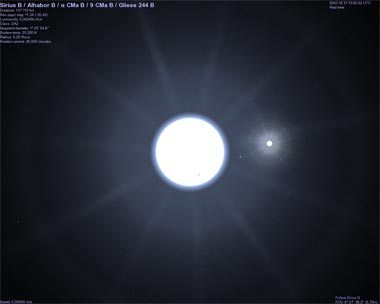
\includegraphics[width=0.5\linewidth]{images/sirius.jpg}
    \caption{\centering Sirius (big white star) and Sirius B (small white star)\\ Source: \url{https://www.estrellasyborrascas.com/images/cieloytierra/foto7.jpg}}
    \label{fig:sirius}
\end{figure}

However, classical physics was not able to cope with the high density of white dwarfs. According to classical physics, such stars would collapse: a new theory is needed.

In 1920 Arthur Eddington hypothesized that stars get their energy from nuclear fusion. In 1925 Pauli stated his eponymous principle for the first time, adding degeneracy pressure from fermions such as electrons as a possible means to stabilize a star. In 1928 Yakov Il'ich Frenkel, a Soviet condensed matter physicist, applied electron Fermi gas theory (a gas theory based on degeneracy pressure) to very dense objects such as white dwarfs. Using this developments E. C. Stoner, another condensed matter physicist from England, deduced in 1929 a mass limit for an ideal uniform density star above which the star would collapse. Finally a mass limit for real white dwarfs was independently calculated in 1931 by Subrahmanyan Chandrasekhar, an Indian-American theoretical physicist.

However, the existence of such a limit implied that stars surpassing it would collapse to a single point. Many physicists at the time, most notably Arthur Eddington, refused this finding as their theories could not explain what happens beyond the limit. Eddington  was very respected and renowned, knew Chandrasekhar personally and was familiar with his works but his opposition to his findings was immense. In fact, in a 1935 meeting of the Royal Astronomical Society, of which both were part, Eddington planned a talk just after Chandrasekhar's in which he criticized and openly ridiculed Chandrasekhar's theory. Moreover, he gave many similar talks in the following years with the same purpose and mean intent.

Despite Eddington's criticisms, Chandrasekhar wrote letters defending his theory to Léon Rosenfeld, Niels Bohr and Wolfgang Pauli among others and received their support. As quantum mechanics advanced, the tide slowly turned to Chandrasekhar's favour. The detection of X-rays from Cygnus X-1 in 1972, the first source widely accepted to be a black hole, meant that Chandrasekhar was right: stars can collapse after all. In 1983 he received half a Nobel Prize for his work.

\subsection{Neutron stars}
In 1933, only two years after the discovery of the neutron, the existence of neutron stars was proposed in a meeting of the American Physical Society by Walter Baade and Fritz Zwicky. In 1939  J. R. Oppenheimer and G. M. Volkoff using recent theoretical developments by Tolman approximately calculated the Tolman-Oppenheimer-Volkov (TOV) limit \cite{oppenheimerMassiveNeutronCores1939} and used it to calculate the TOV limit, which is the neutron star equivalent to the Chandrasekar limit.

Nevertheless, there was no known way to confirm experimentally the existence of such stars until in 1967 when Franco Pacini, an Italian astronomer, hypothesized the phenomenon of pulsars. A pulsar is a highly magnetized and very rapidly spinning neutron star that, according to Pacini, would emit EM radiation. In 1965 Antony Hewish, a British radioastronomer, and Samuel Okoye, a Nigerian astrophysicist, discovered a strange periodic radiation emanating the Crab Nebula, and many similar observations followed. These were later shown to be pulsars, confirming Pacini's theory and the existance of neutron stars. 

\begin{figure}
    \centering
    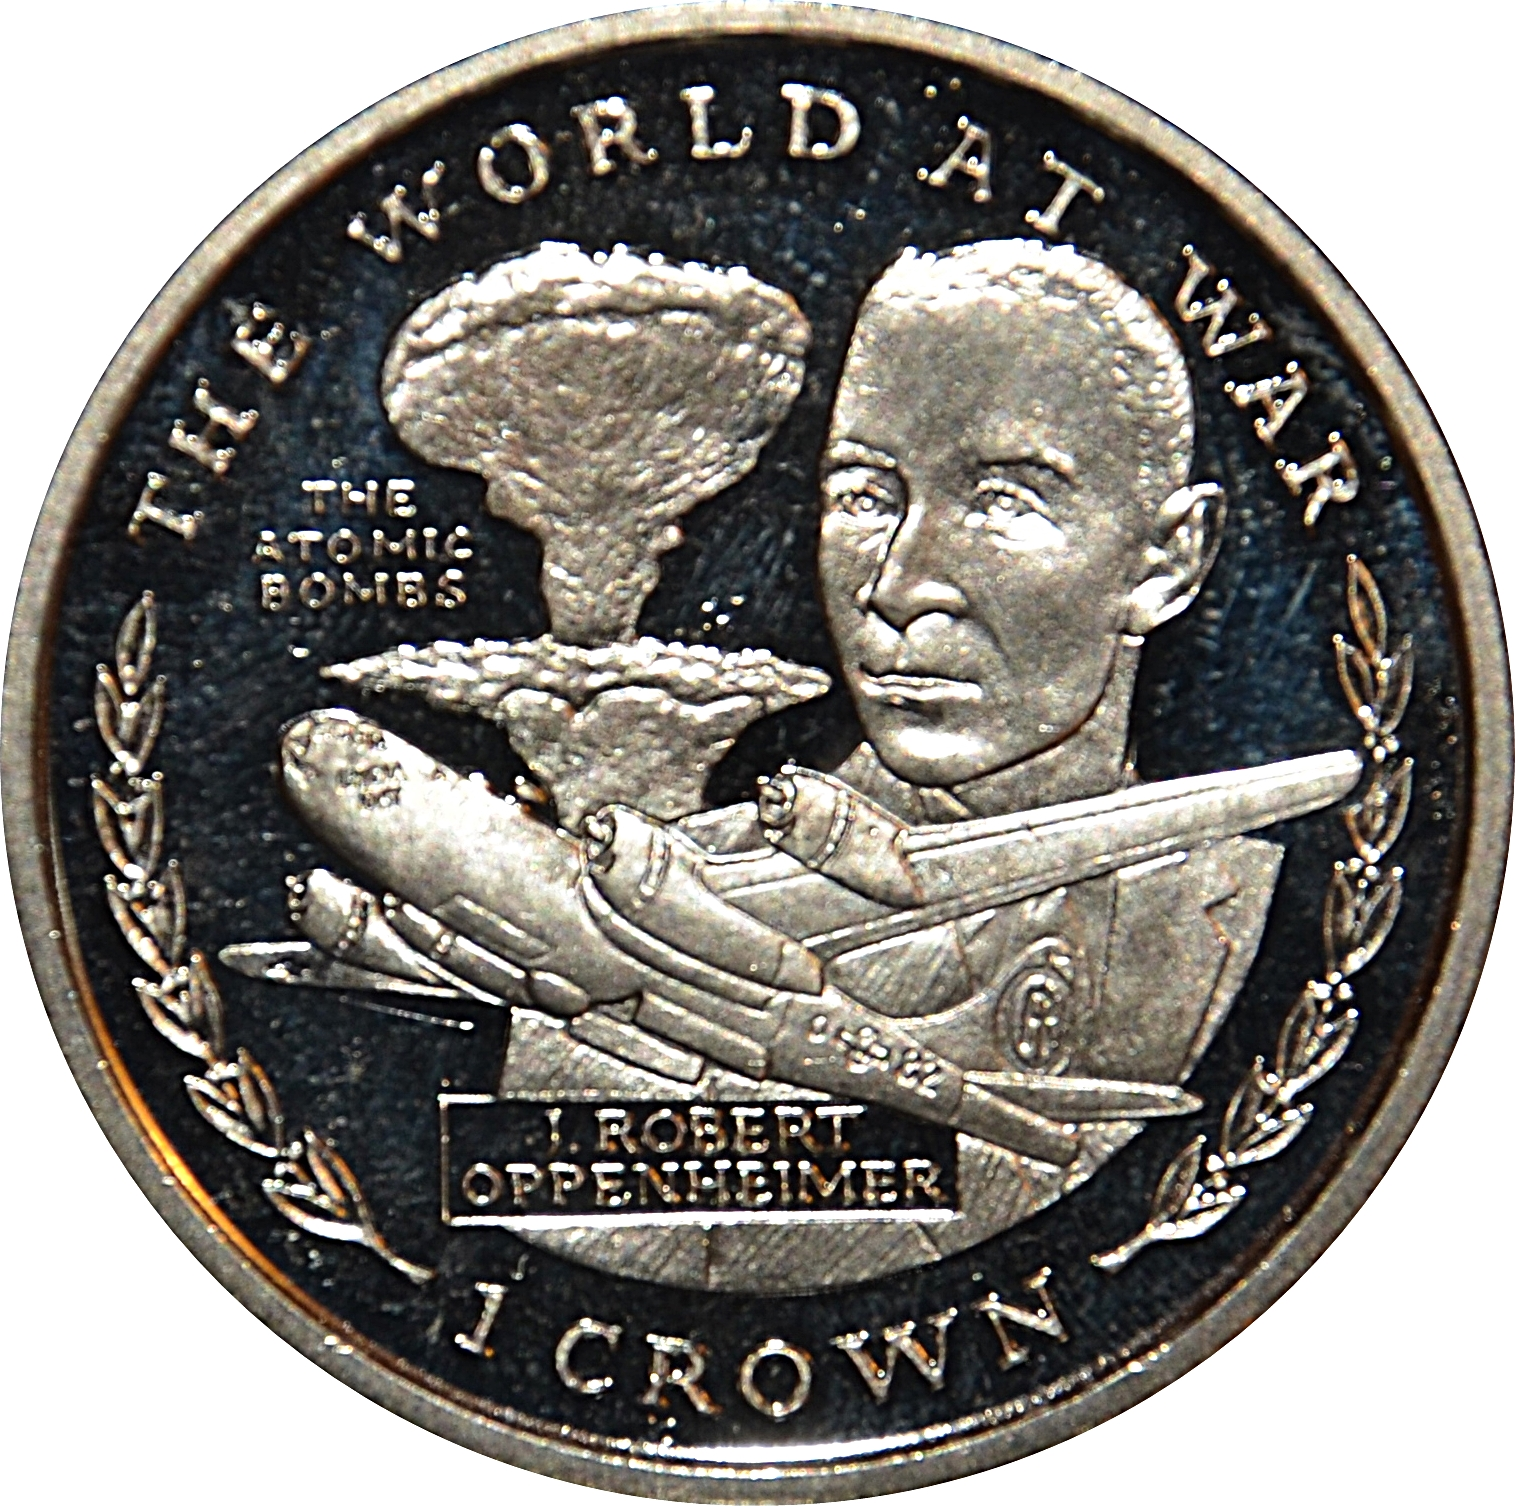
\includegraphics[width=0.3\linewidth]{images/Oppenheimer_coin.jpg}
    \caption{\centering Commemorative 1 crown coin with Oppenheimer (Gibraltar 1999)\\ Source: \url{https://es.numista.com/catalogue/pieces195857.html}}
    \label{fig:oppenheimercoin}
\end{figure}

\section{Compact stars} \label{sec:compactstars}
When a star has burnt all of its hydrogen and helium, a core of carbon, silicon or iron (or sometimes other elements) is formed. As the remaining fuel in the core is exhausted, thermal pressure decreases and gravity pushes particles together until they fall to the lowest energy quantum states possible. Yet the Pauli principle prevents two fermions of falling to the same quantum state,\footnote{Particles can be categorized into two groups depending on their spin. A \textit{fermion} is any particle with half-integer spin (such as electrons, protons and neutrons) and a \textit{boson} is any particle with an integer spin (such as photons). In contrast to bosons, fermions obey the Pauli exclusion principle which states that two identical particles cannot occupy the same quantum state.} so a degeneracy pressure shows up to prevent this. This pressure exists even at absolute zero temperature.

If the gravitational pressure is greater than the degeneracy pressure, the star will collapse and form a black hole.

Conversely, if the degeneracy pressure is sufficient to stabilize stars against gravitational attraction a degenerate star is created. There are two known types of degenerate star: white dwarfs and neutron stars. White dwarfs have an electron degeneracy pressure preventing electrons with parallel spins of falling to the the same energy level. If this pressure is not strong enough the white dwarfs can collapse into neutron stars which enjoy a stronger neutron degeneracy pressure. 

All this means the mass of degenerate stars has an upper limit beyond which gravitational attraction is stronger than degeneracy pressure. For white dwarfs, this limit is the Chandrasekhar limit. For neutron stars it is the Tolman–Oppenheimer–Volkoff (TOV) limit.

In conclusion, white dwarfs, neutron stars and black holes are the three possible remnants after the life of a star. They are collectively called \textit{compact stars} or \textit{stellar remnants}. This report is devoted to the study of white dwarfs: we will derive and solve various equations relating thermodynamic properties inside the star and we will calculate the Chandrasekhar limit.

\section{Structure equation of a star} \label{sec:structureeq}
 Our goal is to find the pressure $p(r)$ for every point inside the star with distance $r$ from its center. In this section we will derive a differential equation that describes this function.

 The gravitational force felt by a spherical layer of width $\odif{r}$ is, according to Newton's law of universal gravitation:
 \begin{equation} \label{eq:gravforce}
     F_g=-G\frac{\M(r) \rho(r) 4 \pi r^2}{r^2} \odif{r}=- 4 \pi G \M(r) \rho(r) \odif{r}
 \end{equation}
 where $\M(r)$ is the mass inside a spherical surface of radius $r$ and $\rho(r)$ is mass density at radius $r$ which is assumed to be spherically symmetric.  As it is explained in \cite{tipler_mosca}, we need not consider the mass outside the sphere of radius $r$.
 
 If the mass inside the star is at rest, the resulting force felt by the spherical layer must be 0. Therefore, if we consider the surface of the spherical layer \(s\) to be the same inside and out we get:
 \begin{align*}
      -sp(r+\odif{r})+sp(r) - F_g & = 0 \\
      sp(r+\odif{r})-sp(r) & = F_g
\end{align*}
Using $s=4 \pi r^2$ and equation \eqref{eq:gravforce}:
\begin{align*}
     4 \pi r^2 p(r+\odif{r})- 4 \pi r^2 p(r) & = -4 \pi G \M(r)\rho(r)  \odif{r} \\
     p(r+\odif{r}) -p(r) & = -\frac{G\M(r)\rho(r)}{r^2} \odif{r} \\
 \end{align*}
Which gives us the derivative of $p(r)$. We have obtained the \textit{hydrostatic equilibrium structure equation}:
 \begin{equation} \label{eq:structure}
     \odv{p}{r} = -\frac{G\M(r)\rho(r)}{r^2} = -\frac{G\M(r)\epsilon(r)}{c^2 r^2}
 \end{equation}
 Mass $\M$ inside the sphere can be found by integrating
 \begin{equation} \label{eq:massinsphere}
     \odv{\M}{r} = 4 \pi r^2 \rho(r) = 4 \pi r^2 \frac{\epsilon(r)}{c^2}
 \end{equation}
The second half of these equations is obtained using special relativity's rest mass energy equation $\epsilon = \rho c^2$ where $\epsilon(r)$ is the energy density.

Equation \eqref{eq:structure} does not consider general relativistic effects which are important for bigger stars. The Tolman–Oppenheimer–Volkoff (TOV) equation is a structure equation analogous to equation \eqref{eq:structure} but takes into account general (and special) relativity.
 \begin{equation} \label{eq:tov}
     \odv{p}{r}= -\frac{G\M(r)\epsilon(r)}{c^2 r^2} \left(1+\frac{p(r)}{\epsilon(r)}\right)
     \left(1+\frac{4 \pi r^3 p(r)}{\M(r)c^2}\right)
     \left(1-\frac{2G\M(r)}{rc^2}\right)^{-1}
 \end{equation}
The first two additional terms are special relativistic corrections and the last term is a general relativistic correction whose importance depends on the size of $\frac{G\M(r)}{rc^2}$.

To obtain $\M(r)$ and solve any of the structure equations (\eqref{eq:structure} or \eqref{eq:tov}) we must know the relation between $\epsilon$ and $p$ which is given by the equation of state (EoS) of the star.

In \autoref{sec:eos} we will deduce the EoS and from there we will solve the structure equation for white dwarf stars.


\section[Equation of state for white dwarfs]{Equation of state for white dwarfs \footnote{This chapter is particularly related to the work in \cite{silbarNeutronStarsUndergraduates2004}}} \label{sec:eos}

A Fermi gas is an idealized model composed of many non-interacting fermions in a constant potential. Among other things, it can be used to model electrons in a white dwarf or neutrons in a neutron star. In this section we will treat the inside a white dwarf as a Fermi gas of electrons to deduce an equation of state for the inside of the star. As explained in \autoref{sec:structureeq}, the equation of state relates the energy density $\epsilon$ with pressure $p$.

Number of available electrons $\odif{n}$ at momentum between $k$ and $k+\odif{k}$ per unit volume is \cite{pathria_beale}
\begin{equation} \label{eq:electrondndk}
    \odif{n} = \frac{4\pi k^2 \odif{k}}{(2\pi\hbar)^3}
\end{equation}

An electron can have two spin states for every energy level so we must multiply by 2 and then integrate to find the electrons per unit volume:
\begin{equation} \label{eq:4}
    n = \frac{8\pi}{(2\pi\hbar)^3}\int^{k_F}_{0}k^2 \odif{k} = \frac{k_F^3}{3\pi^2\hbar^3}
\end{equation}
where $k_F$ is the Fermi momentum. $k_F c$ is the Fermi energy which is defined as the difference between the highest and lowest occupied quantum states. Therefore $k_F$ is the maximum momentum electrons can have. 

There is a proton and around one neutron for each electron. If we all nucleons have the same mass $m_N$ and we neglect the mass of the electron, the mass density of the gas is
\begin{equation} \label{eq:3}
    \rho = n m_N \frac{A}{Z}
\end{equation}
If we consider the nucleons to be static, the energy density will be
\begin{equation} \label{eq:1}
    \epsilon = \rho c^2 + \epsilon_e
\end{equation}
We will now deduce the electron energy density $\epsilon_e$.
The energy of one electron is
\begin{equation}
    E_e = (k^2c^2+m_e^2c^4)^{1/2}
\end{equation}
Then, the energy of $\odif{n}$ electrons is 
\begin{equation}
    \odif{\epsilon_e} = E_e \odif{n} = (k^2c^2+m_e^2c^4)^{1/2} \odif{n}=    \odif{\epsilon_e} = (k^2c^2+m_e^2c^4)^{1/2} \frac{8\pi k^2}{(2\pi\hbar)^3}\odif{k}
\end{equation}
From equation \eqref{eq:electrondndk} we get the energy per unit volume associated to the electrons of momentum between $k$ and $k+\odif{k}$
\begin{equation}
    \odif{\epsilon_e} = (k^2c^2+m_e^2c^4)^{1/2} \frac{8\pi k^2}{(2\pi\hbar)^3}\odif{k}
\end{equation}
To find the energy per unit volume we integrate for all the electrons that have all the possible values for the momentum. We apply the change of variables 
$u = \frac{k}{m_ec} \implies \odif{k} = m_e c \odif{u}$
and we find the corresponding primitive using \href{https://www.integral-calculator.com}{integral-calculator.com}.
\begin{align*} 
    \epsilon_e(k_F) & = \int^{k_F}_{0} (k^2c^2+m_e^2c^4)^{1/2} \frac{8\pi k^2}{(2\pi\hbar)^3}\odif{k} \\
    & = \frac{8\pi}{(2\pi\hbar)^3} \int^{k_F}_{0} (k^2c^2+m_e^2c^4)^{1/2} k^2 \odif{k}\\
    & = \frac{8\pi}{(2\pi\hbar)^3} \int^{\frac{k_F}{m_ec}}_{0} (u^2m_e^2c^4+m_e^2c^4)^{1/2} u^2 m_e^2 c^2 m_e c \odif{k}\\
    & = \frac{8\pi}{(2\pi\hbar)^3} m_e^4c^5 \int^{\frac{k_F}{m_ec}}_{0} (u^2+1)^{1/2} u^2 \odif{k}\\
    & = \epsilon_0 \int^{\frac{k_F}{m_ec}}_{0} (u^2+1)^{1/2} u^2 \odif{k}\\ 
    & = \frac{\epsilon_0}{8} \left[(x^2+1)^{1/2}(2x^3+x)-\asinh(x)\right] \numberthis \label{eq:2}
\end{align*}
where $\epsilon_0 = \frac{m_e^4c^5}{\pi^2\hbar^3}$ and $x = x(k_F) = \frac{k_F}{m_ec}$. 
Then the total energy density
\begin{equation}
    \epsilon = n m_N \frac{A}{Z} + e_e(k_F)
\end{equation}

Now that we know $\epsilon$, to get the EoS we need an equation for $p$. From the first law of thermodynamics $\odif{U} = \fdif{Q} - p\odif{V}$ we know
\begin{equation} \label{eq:termo1}
    p=-\pdv[delims-eval=.|]{U}{V}_{T = 0}
\end{equation}
For a unit of volume, the energy per electron is $\epsilon/n$ and the volume per electron is
\begin{equation}
    V = \frac{1}{n} \Longrightarrow \odv{V}{n} = -\frac{1}{n^2} \Longrightarrow \odif{V} = -\frac{\odif{n}}{n^2}
\end{equation}
Substituting in equation \eqref{eq:termo1} we get
\begin{equation}
    p = - \frac{\odif{\left(\frac{\epsilon}{n}\right)}}{-\frac{\odif{n}}{n^2}} = n^2\frac{\odif{\left(\frac{\epsilon}{n}\right)}}{\odif{n}} = n^2\frac{\odv{\epsilon}{n}n-\epsilon}{n^2} = \odv{\epsilon}{n}n-\epsilon
\end{equation}
Using equation \eqref{eq:1} and substituting equations \eqref{eq:3} and \eqref{eq:2}
\begin{equation} \label{eq:15}
    \frac{\epsilon}{n} = m_N A/Z + \frac{1}{n}\epsilon_e(k_F)
\end{equation}
Then
\begin{gather*}
     p = n^2 \odv*{\left(\frac{\epsilon}{n}\right)}{n}\\
     = 0 + n^2\odv*{\left(\frac{\epsilon_e(k_F)}{n}\right)}{n}\\
    = n^2\odv*{\left(\frac{1}{n} \frac{8\pi}{(2\pi\hbar)^3} \int^{k_F}_{0} (k^2c^2+m_e^2c^4)^{1/2} k^2 \odif{k}\right)}{n}\\
    = n^2\left(-\frac{1}{n^2} \frac{8\pi}{(2\pi\hbar)^3}  \int^{k_F}_{0} (k^2c^2+m_e^2c^4)^{1/2} k^2  \odif{k} + \frac{1}{n} \frac{8\pi}{(2\pi\hbar)^3} \odv*{\left(\int^{k_F}_{0}(k^2c^2+m_e^2c^4)^{1/2} k^2 \odif{k} \right)}{n}\right) \\
\end{gather*}

We know that $k_F$ depends on n as in equation \eqref{eq:electrondndk}. Therefore, we can differentiate the second term inside the bracket using the first fundamental theorem of calculus \cite{spivak}.

\begin{gather*}
    \frac{\frac{8\pi}{(2\pi\hbar)^3} }{n} \odv*{\left(\int^{k_F}_{0}(k^2c^2+m_e^2c^4)^{1/2} k^2 \odif{k} \right)}{n}  = \frac{\frac{8\pi}{(2\pi\hbar)^3} }{n}(k_F^2c^2+m_e^2c^4)^{1/2} k_F^2 \odv{k_F}{n}\\
    = \frac{\frac{8\pi}{(2\pi\hbar)^3} }{n}(k_F^2c^2+m_e^2c^4)^{1/2} k_F^2 \frac{\pi^2\hbar^3}{k_F^2}
    = \frac{\frac{8\pi}{(2\pi\hbar)^3} }{n^2} \frac{k_F^3}{3\pi^2\hbar^3}
    (k_F^2c^2+m_e^2c^4)^{1/2} \pi^2\hbar^3\\
    = \frac{\frac{8\pi}{(2\pi\hbar)^3} }{3 n^2}
    (k_F^2c^2+m_e^2c^4)^{1/2} k_F^3 \\
\end{gather*}

Defining
\begin{gather*}
    v(k) \equiv (k^2c^2+m_e^2c^4)^{1/2} \hspace{1cm}
    u(k) \equiv \frac{k^3}{3}
\end{gather*}
we can rewrite the expression for $p$.
\begin{gather*}
    p = \frac{8\pi}{(2\pi\hbar)^3} \left(\left[uv\right]_0^{k_F} - \int^{k_F}_{0}v \odv{u}{k} \odif{k} \right)
    = \frac{8\pi}{3(2\pi\hbar)^3} \int^{k_F}_{0} u \odv{v}{k} \odif{k}
\end{gather*}
and substituting $v(k)$ and $u(k)$, we find a shorter expression for $p$.
\begin{equation} \label{eq:pint}
    p(k_F) = \frac{8\pi}{3(2\pi\hbar)^3} \int^{k_F}_{0}(k^2c^2+m_e^2c^4)^{-1/2} k^4 c^2 \odif{k}
\end{equation}

 It is possible to solve the integral \eqref{eq:pint} using the same change of variables than in \eqref{eq:2} and \href{https://www.integral-calculator.com}{integral-calculator.com} to find the primitive.

\begin{equation}
\begin{split}
        p &= \frac{8\pi}{3(2\pi\hbar)^3} \int^{\frac{k_F}{m_ec}}_{0} (u^2m_e^2c^4+m_e^2c^4)^{-1/2} c^2 u^4 m_e^4 c^4 m_e c \odif{k}\\
        & = \frac{8\pi}{3(2\pi\hbar)^3} m_e^4 c^5 \int^{\frac{k_F}{m_ec}}_{0} (u^2+1)^{-1/2} u^4 \odif{k} \\
        & = \frac{\epsilon_0}{24}\left[(x^2+1)^{1/2}(2x^3-3x)+3\asinh(x)\right]
\end{split}
\end{equation}

where $\epsilon_0 = \frac{m_e^4c^5}{\pi^2\hbar^3}$ and $x = x(k_F) = \frac{k_F}{m_ec}$.

The pressure as a function of the energy density is represented in \autoref{fig:pvsepsilon} for values $0< k_F < 2m_ec$.

\begin{figure}
\centering
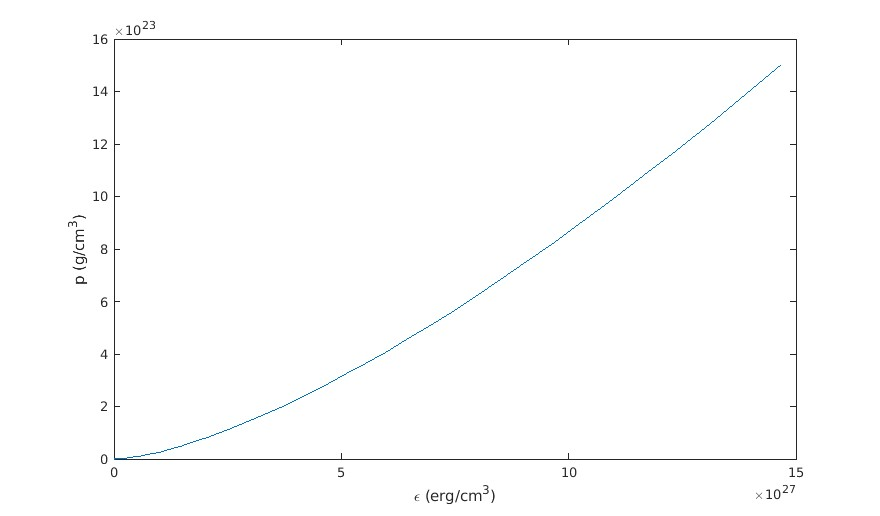
\includegraphics[width=0.6\textwidth]{images/pvsepsilon.jpg}
\caption{Pressure as a function of energy density.}
\label{fig:pvsepsilon}
\end{figure}

\subsection[Relativistic case]{Relativistic case: $k_F\gg m_ec$} \label{sec:relativistic_limit}
It is possible to find a theoretical expression relating energy density $\epsilon$ and pressure $p$ for the case in which the maximum momentum of the electrons $k_F$ is very large. It is the relativistic case. If $k_F\gg m_ec$ then $\frac{k_F}{m_ec}\gg 1$ that implies $\left(\frac{k_F}{m_ec}\right)^2 + 1 \approx \left(\frac{k_F}{m_ec}\right)^2$. Then
\begin{align*}
    p(k_F) &= \frac{\epsilon_0}{3}\int^{\frac{k_F}{m_ec}}_{0} (u^2+1)^{-1/2} u^4 \odif{k} \\
    & = \frac{\epsilon_0}{3}\int^{\frac{k_F}{m_ec}}_{0} u^{-1} u^4 \odif{k}\\
    & = \frac{1}{12} \frac{m_e^4c^5}{\pi^2\hbar^3} \frac{1}{m_e^4c^4}k_F^4 \numberthis
\end{align*}
Using equation \eqref{eq:4} and substituting $n$ from \eqref{eq:3}
\begin{equation} \label{eq:5}
\begin{split}
    p(k_F) &= \frac{1}{12} \frac{m_e^4c^5}{\pi^2\hbar^3} \frac{1}{m_e^4c^4}\hbar^4\left(\frac{3\pi^2\rho Z}{m_NA}\right)^{4/3} \\
    &= \frac{\hbar c}{12 \pi ^2}\left(\frac{3\pi^2\rho Z}{m_NA}\right)^{4/3}
\end{split}
\end{equation}

The assumption $\epsilon = \rho c^2$ is valid if $k_F \ll m_ec\frac{m_N}{m_e}\frac{4A/Z}{3}$. Let's see why this is the case:
\begin{equation}
    \epsilon_e(k_F) = \epsilon_0 \int^{\frac{k_F}{m_ec}}_{0} (u^2+1)^{1/2} u^2 \odif{k}
    = \epsilon_0 \int^{\frac{k_F}{m_ec}}_{0} u^3 \odif{k}
    = \frac{\epsilon_0}{4}\left(\frac{k_F}{m_ec}\right)^4= \frac{k_F^4c}{4\pi^2\hbar^3}
\end{equation}
and
\begin{equation}
    \rho c^2 = nm_NA/Zc^2 = \frac{k_F^3}{3\pi^2\hbar^3}m_NA/Zc^2
\end{equation}
therefore $\rho c^2 \gg  \epsilon_e$ so $\epsilon = \rho c^2$. Substituting this in equation \eqref{eq:5} we get the relativistic structure equation:
\begin{equation} \label{eq:24}
    p = K_{\mathrm{rel}} \epsilon^{4/3}
    \quad \mathrm{where} \quad
    K_{\mathrm{rel}}=
    \frac{\hbar c}{12 \pi ^2}\left(\frac{3\pi^2Z}{Am_Nc^2}\right)^{4/3}
\end{equation}

Constant $K_{\mathrm{rel}}$ has units
\begin{equation}
    \left[\frac{\hbar c}{12 \pi ^2}\left(\frac{3\pi^2Z}{Am_Nc^2}\right)^{4/3}\right] = \frac{\unit{g.cm/s^2}\unit{cm.s}}{\unit{g^{4/3}cm^{5/3}/s^{5/3}}} = \frac{\unit{cm^{1/3}s^{2/3}}}{\unit{g^{1/3}}}
\end{equation}
that are consistent with the units of $p/\epsilon^{4/3}$.

Therefore, we have found an equation of state for the limit $k_F \gg m_ec$.

\subsection[Nonrelativistic case]{Nonrelativistic case: $k_F \ll m_ec$}

It is also possible to find an analogous expression to the one found in \ref{sec:relativistic_limit} for the case in which the maximum momentum of the electrons $k_F$ is very small. It is the nonrelativistic case. 
If $k_F\ll m_ec$ then $\frac{k_F}{m_ec}\ll1$ that implies $\left(\frac{k_F}{m_ec}\right)^2 + 1 \approx 1$. Then
\begin{equation}
\begin{split}
    p(k_F) &= \frac{\epsilon_0}{3}\int^{\frac{k_F}{m_ec}}_{0} (u^2+1)^{-1/2} u^4 \odif{k} \\
    & = \frac{\epsilon_0}{3}\int^{\frac{k_F}{m_ec}}_{0} 1 u^4 \odif{k}\\
    & = \frac{1}{15} \frac{m_e^4c^5}{\pi^2\hbar^3} \frac{1}{m_e^5c^5}k_F^5
\end{split}
\end{equation}
Using equation \eqref{eq:4} and substituting $n$ from \eqref{eq:3}
\begin{equation} \label{eq:6}
\begin{split}
    p(k_F) &= \frac{1}{15} \frac{m_e^4c^5}{\pi^2\hbar^3} \frac{1}{m_e^5c^5}\hbar^5\left(\frac{3\pi^2\rho Z}{Am_N}\right)^{5/3} \\
    &= \frac{\hbar^2 }{15 \pi ^2 m_e}\left(\frac{3\pi^2\rho Z}{m_NA}\right)^{5/3}
\end{split}
\end{equation}

Since $m_e \ll m_N A/Z$, we can again assume $\epsilon = \rho c^2$:
\begin{equation}
\begin{split}
    \epsilon_e(k_F) &= \epsilon_0 \int^{\frac{k_F}{m_ec}}_{0} (u^2+1)^{1/2} u^2 \odif{k}\\
    & = \epsilon_0 \int^{\frac{k_F}{m_ec}}_{0} 1u^2 \odif{k}\\
    & = \frac{\epsilon_0}{3}\left(\frac{k_F}{m_ec}\right)^3\\    & = \frac{m_e c^2}{3\pi^2\hbar^3}k_F^3
\end{split}
\end{equation}
and
\begin{equation*}
    \rho c^2 =\frac{m_N A c^2}{3\pi^2\hbar^3Z}k_F^3 
\end{equation*}
therefore $\epsilon_e(k_F) \ll  \rho c^2$ and $\epsilon=\rho c^2$. Substituting this in equation \eqref{eq:6} we get the nonrelativistic structure equation:
\begin{equation} \label{eq:30}
    p =  K_{\mathrm{nonrel}} \epsilon^{5/3} \quad \mathrm{where} \quad K_{\mathrm{nonrel}}=\frac{\hbar^2 }{15 \pi ^2 m_e}\left(\frac{3\pi^2Z}{Am_Nc^2}\right)^{5/3}
\end{equation}

The units of the constant $K_{\mathrm{nonrel}}$ are:
\begin{equation}
    \left[\frac{\hbar^2 }{15 \pi ^2 m_e}\left(\frac{3\pi^2Z}{Am_Nc^2}\right)^{5/3}\right] = \frac{\unit{g^2cm^2/s^4}\unit{cm^2/s^2}}{\unit{g^{8/3}cm^{10/3}/s^{10/3}}} = \frac{\unit{cm^{2/3}s^{4/3}}}{\unit{g^{2/3}}}
\end{equation}
that is consistent with the units of $p/\epsilon^{5/3}$.

In short, we have found an equation of state for the limit $k_F \ll m_ec$.

\section{Solving the structure equation for white dwarfs} \label{sec:solvingstructure}

Now that we have an equation of state we are able to solve the structure equations (ODEs) presented on \autoref{sec:structureeq}, namely:
\begin{equation} \tag{\ref{eq:structure}}
    \odv{p}{r} = -G\frac{\epsilon(r)\M(r)}{c^2r^2}
\end{equation}
\begin{equation} \tag{\ref{eq:massinsphere}}
    \odv{\M}{r} = \frac{4\pi r^2\epsilon(r)}{c^2}
\end{equation}
A typical white dwarf has mass $M<1.4 \Msun$ and radius $R\sim \qty{e4}{km}$ which means $\frac{GM}{c^2R} \sim \num{e-4}$. Therefore we can safely omit general relativistic effects and use the nonrelativistic structure equation \eqref{eq:structure}.

To simplify things, we can express mass in terms of our Sun's mass  $\Mbar(r) = {\M}(r)/\Msun $ and use dimensionless factors $\bar{\epsilon} = \epsilon/\epsilon_{0}$ and $\bar{p} = p/\epsilon_{0}$ well defined as $\epsilon$ and $p$ have the same dimensions (choosing $\epsilon_0$ whith suitable units). But what is really going to let us solve the ODEs is the relation found in equations \eqref{eq:24} and \eqref{eq:30}, from which we can write
\begin{equation}
    p = K\epsilon^{\gamma} \implies \epsilon = \left(\frac{p}{K}\right)^{1/\gamma}
\end{equation}
Stars with such an equation of state are called polytropes. Now we can rewrite equations \eqref{eq:structure} and \eqref{eq:massinsphere} 
\begin{equation}
    \odv{\bar{p}(r)}{r} = -G\frac{\Msun }{c^2}\frac{\epsilon_0^{1/\gamma}\bar{p}(r)^{1/\gamma}\Mbar(r)}{\epsilon_0 K^{1/\gamma}r^2} = -\mathcal{A}\epsilon_0^{\frac{1-\gamma}{\gamma}}\frac{\bar{p}(r)^{1/\gamma}\Mbar(r)}{r^2}
\end{equation}
\begin{equation}
    \odv{\Mbar(r)}{r} = \frac{4\pi}{\Msun c^2} r^2\left(\frac{\epsilon_0}{K}\right)^{1/\gamma}\bar{p}(r)^{1/\gamma} = \mathcal{B}\epsilon_0^{1/\gamma}r^2\bar{p}(r)^{1/\gamma}
\end{equation}
where $\mathcal{A} \equiv G\frac{\Msun }{c^2K^{1/\gamma}} $ and $\mathcal{B} \equiv \frac{4\pi}{\Msun c^2 K^{1/\gamma}}$. 

\subsection[Relativistic case]{Relativistic case: $k_F \gg  m_e c$} \label{subsec:solvingrel}

Let's solve first the relativistic case using the EoS \eqref{eq:24}, i.e. taking $\gamma = 4/3$, setting
\[K \equiv K_{\mathrm{rel}} =
\frac{\hbar c}{12 \pi ^2}\left(\frac{3\pi^2}{A/Zm_Nc^2}\right)^{4/3} 
=\qty{1.0038e-13}{m/J^{1/3}}
=\qty{0.61981}{km/(\Msunc)^{1/3}}\]
and choosing the numerical value of $\epsilon_0$, for which we will follow the recommendation of  \cite{silbarNeutronStarsUndergraduates2004} and take $\epsilon_0 = \qty{4.17}{\Msunc/km^3}$. We have $\mathcal{A} = \qty{2.1241}{km^{1/4} (\Msunc)^{1/4}}$ and $\mathcal{B} = \qty{17.9894}{km^{-3/4}(\Msunc)^{-3/4}}$ so we can solve
\begin{equation} \label{eq:37}
    \odv{\bar{p}(r)}{r} = -\alpha~ \frac{\bar{p}(r)^{1/\gamma}\Mbar(r)}{r^2} 
    \quad \mathrm{and} \quad
    \odv{\Mbar(r)}{r} = \beta r^2\bar{p}(r)^{1/\gamma}
\end{equation}
with $\alpha = \mathcal{A}\epsilon_0^{\frac{1-\gamma}{\gamma}} = \qty{1.486}{km}$ and $\beta = \mathcal{B}\epsilon_0^{1/\gamma} = \qty{52.495}{km^{-3}}$.

Now we will integrate the coupled ODEs system using a Runge-Kutta-Fehlberg method included in the SciPy Python library.  The upper limit of integration $r = R$ is the unknown radius of the star, but we do not need to know it because the program will stop itself around the maximum radius. The way it does it is to calculate solutions for intervals, inside a do-loop the program solves the ODEs between $r$ and $r + \adif{r}$ and checks the value of $\bar{p}(r + \adif{r})$. If it has turned negative (or negligible) the program stops, otherwise it continues integrating the next interval ($r + \adif{r}$, $r + 2\adif{r}$). When the pressure vanishes (it is very small in comparison to $\bar{p}(0)$) we understand that the star does not longer exist in that region.

Using this program and taking as initial conditions $\Mbar(0) = 0$ and $\bar{p}(0) = \num{1e-15}$ we get the next distributions of $\Mbar$ (in $\Msun $) and $\bar{p}$ (dimensionless) in terms of the radius (km): 
\begin{figure}[h]
    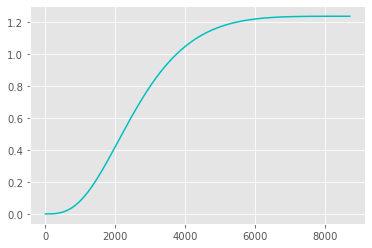
\includegraphics[width=7.3cm]{images/M-r Rel.png}
    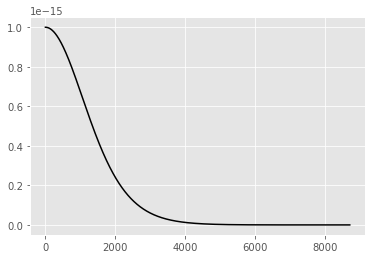
\includegraphics[width=7.3cm]{images/p-r Rel.png}
    \centering
    \caption{$\Mbar(r)$ and $\bar{p}(r)$ for $\bar{p}(0) =\num{1e-16}$ in the relativistic case.}\label{fig:Relativistic}
\end{figure}

As seen in \autoref{fig:Relativistic} the mass  converges to a limit for large $r$. The star radius is about $R = \qty{8300}{km} \simeq 0.012 \symrm{R}_\odot$, which fits our expectations. Pressure becomes very small and practically constant after approximately $R/2$.

This results are intuitively strongly dependent on our choice of $\bar{p}(0)$. To see this relation we can plot the white dwarf's radius and maximum mass in terms of $\bar{p}(0)$ (the last radius for which the program have solved the ODE and the mass calculated there):

\begin{figure}[h]
    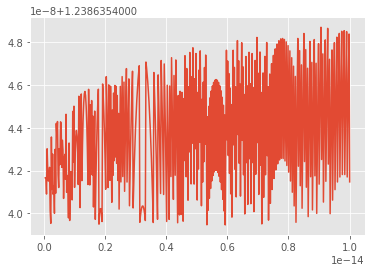
\includegraphics[width=7.3cm]{images/M-p0.png}
    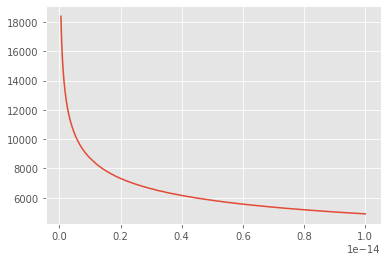
\includegraphics[width=7.3cm]{images/R-p0.png}
    \centering
    \caption{$\Mbar$ and $R$ (in km) in terms of $\bar{p}(0)$ in the relativistic case.}
\label{fig:Comparison}
\end{figure}

From this results we can draw a few conclusions. 

First, the mass of the star does not depend on the initial pressure. The $Y$-axis (mass) scale is $1.2386 + y\cdot 10^{-8}$ with $y \in (3.8, 5)$ so that $\Mbar \approx 1.2386$ which is a fair approximation.

Second, the radius decreases rapidly as $\bar{p}(0)$ increases for pressures between $\num{.5e-16}$ and $\num{1e-15}$,\footnote{$\bar{p}(0)$ was limited to $[\num{0.5e-16}, \num{1e-14}]$} and from there the behaviour is more much more controlled. Thus, for larger $\bar{p}(0)$ the star will be more compact but not more massive. Even so, it can be seen that for large enough values to $\bar{p}(0)$  the radius tends to 0, so its value is not limited. Therefore not any election of $\bar{p}(0)$ will give a correct or physically feasible star model.


As an additional comment, thereby justifying that tendency of the radius, it can be deduced from the analytical solution of the problem \cite{silbarNeutronStarsUndergraduates2004} that $R \propto \bar{p}(0)^{-1/4}$ and we can see it clearly in \autoref{fig:6}, where the blue curve is $\bar{p}(0)^{-1/4}$ therefore $R \to 0$.

\begin{figure}[h]
    \centering
    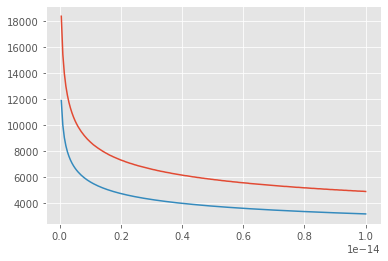
\includegraphics[width=8cm]{images/r-r^0.25-p0.png}
     \caption{Radius vs. $\bar{p}(0) ~\&~ \bar{p}(0)^{-1/4}$}
     \label{fig:6}
\end{figure}

\subsection[Nonrelativistic case]{Nonrelativistic case: $k_F \ll m_e c$} \label{subsec:solvingnonrel}

To solve the nonrelativistic case we will follow the same strategy, changing only the value of $\gamma = 5/3$, setting
\[K \equiv K_{\mathrm{nonrel}} = \frac{\hbar^2}{15 \pi ^2 m_e}\left(\frac{3\pi^2}{A/Zm_Nc^2}\right)^{5/3} = \qty{1.5317252e-22}{m^2 J^{-2/3}} = \qty{4859.065}{km^2 (\Msunc)^{-2/3}}\]
and $\epsilon_0 =\qty{0.014}{\Msunc/km^3}$. $\gamma$ and $K$ come from \eqref{eq:30} and $\epsilon_0$ is again a value from \cite{silbarNeutronStarsUndergraduates2004}. Substituting in \eqref{eq:37} (see \autoref{sec:codes} for the code used) and using $\bar{p}(0) = \num{1e-16}$ we get the results in \autoref{fig:nonrelativistic}.

\begin{figure}[h]
    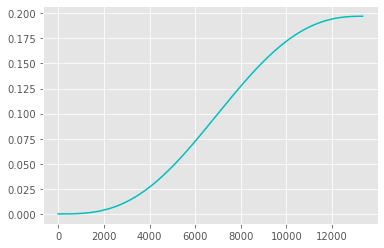
\includegraphics[width=7.3cm]{images/M-r Non-rel (2).png}
    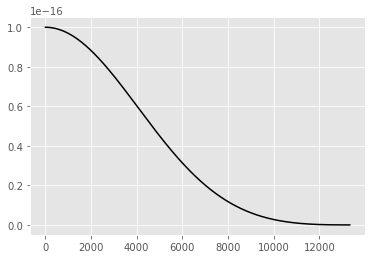
\includegraphics[width=7.3cm]{images/p-r Non-Rel (2).png}
    \centering
    \caption{$\Mbar(r)$ and $\bar{p}(r)$ for $\bar{p}(0) = 1\cdot 10^{-16}$ in the nonrelativistic case.}
    \label{fig:nonrelativistic}
\end{figure}

The most obvious differences from \autoref{fig:Relativistic} are the small value of the mass and the rapid decrease of the pressure. The curve does not end in a long flat line in  any of the cases. \autoref{fig:Comparison2} shows again the mass and radius of the star for each value of $\bar{p}(0)$.

\begin{figure}[h]
    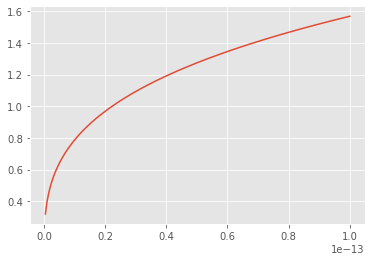
\includegraphics[width=7.3cm]{images/M-p0 Non-rel.png}
    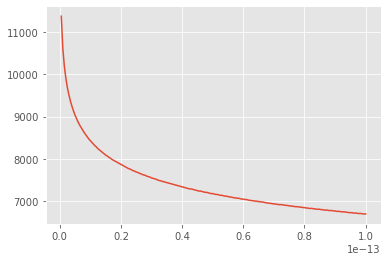
\includegraphics[width=7.3cm]{images/R-p0 Non-Rel.png}
    \centering
    \caption{$\Mbar$ and $R$ (in km) in terms of $\bar{p}(0)$ in the nonrelativistic case}
\label{fig:Comparison2}
\end{figure}

The limits for $\bar{p}(0)$ were $[\num{0.5e-15}, \num{1e-13}]$. The radius again tends to zero but now the mass does not appear to have a limit. The reason for that is the high range of values of $\bar{p}(0)$ considered, because for $\bar{p}(0) > \num{e-14}$ the nonrelativistic assumption does not work and hence these plots have no physical meaning.

In the next section we aim to join the meaningful intervals of each limit to obtain a general solution.

\subsection{General solution} \label{subsec:solvinggeneral}

We want a good approximation that fits for every value of $\bar{p}(0)$, relativistic or not. Taking as a hint the two expressions for each limit developed in the previous lines (and the suggestion of \cite{silbarNeutronStarsUndergraduates2004}) we will search for a general solution of the form:
\begin{equation} \label{eq:38}
    \bar{\epsilon}(\bar{p}) = X_{\mathrm{nonrel}}\bar{p}^{3/5} + X_{\mathrm{rel}}\bar{p}^{3/4}
\end{equation}
Rewriting equations \eqref{eq:15} and \eqref{eq:pint} in terms of $x = k_F/m_e c$:
\begin{equation}
    \epsilon(x) = \frac{\epsilon_0}{8}((2x^3 + x)(1+x^2)^{1/2} - \asinh{x}) + \frac{m_N A/Z c^2}{3\pi^2 \hbar^3}(xm_ec)^3
\end{equation}
\begin{equation}
    p (x) = \frac{\epsilon_0}{24}((2x^3 - 3x)(1+x^2)^{1/2} + 3\asinh(x))
\end{equation}
The lest term of $\epsilon$ comes from \eqref{eq:4}. This are the ones used to plot \autoref{fig:pvsepsilon}. Now we should search for $X_{\mathrm{nonrel}}$ and $X_\mathrm{rel}$ so that \eqref{eq:38} fits the curve $(\epsilon/\epsilon(0),\space p/\epsilon(0))_x$ where $k_F \in (0, 2m_e c)$. For this purpose, we have used the built-in fitting function of \texttt{scipy.optimize} and the results are: 

\begin{equation} \label{eq:41}
    X_{\mathrm{nonrel}} = 0.0303956 \quad \mathrm{and} \quad  X_{\mathrm{rel}} = 3.51136
\end{equation}
with an estimated standard deviation of $\num{3.97447998e-5}$ and $\num{3.63361223e-3}$ respectively (given by the function), so it is then a good approximation of the curve.

With this solutions the odes to solve are:
\begin{equation}
    \odv{\bar{p}}{r} = -G\frac{\Msun }{c^2}\frac{\bar{\epsilon}(\bar{p})\Mbar(r)}{r^2} = -R_0 \frac{\bar{\epsilon}(\bar{p})\Mbar(r)}{r^2}
\end{equation}
\begin{equation}
    \odv{\Mbar(r)}{r} = \frac{4\pi}{\Msun c^2} r^2 \epsilon_0 \bar{\epsilon}(\bar{p}) = \beta r^2 \bar{\epsilon}(\bar{p})
\end{equation}
where $R_0 = -G\frac{M_\odot}{c^2} = \qty{1.4767}{km}$ and $\beta = 4\pi \epsilon_0/M_\odot c^2$.

Choosing, for reasons of numerical stability of the ODE solver,
\[\epsilon_0 = \qty{1e-37}{erg/cm^3} = \qty{0.0055954}{ \Msunc/km^3}\]
then $\beta = \qty{0.070314}{km^{-3}}$.  We solve as in the previous sections, now with a larger interval of values for $\bar{p}(0)$ ($[\num{0.5e-16},\num{e-10}]$) and get the following graphs:

\begin{figure}[h]
    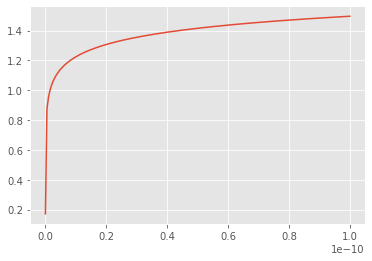
\includegraphics[width=7.3cm]{images/M-p0 gen.png}
    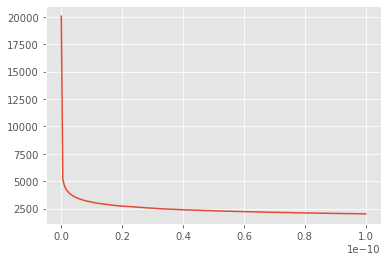
\includegraphics[width=7.3cm]{images/R-p0 gen.png}
    \centering
    \caption{$\Mbar$ and $R$ (in km) in terms of $\bar{p}(0)$ for an approximated general solution or $\epsilon(p)$}
\label{fig:Comparison3}
\end{figure}

In the radius graph one cannot see very much, as it decreases almost vertical for small initial pressures and then it has a flat form from $\num{3e-11}$ to the end of the graph. Nevertheless, something interesting is the fact that it does not tend to $0$, or at least that tendency is much slower (the graph is flatter). 

About the mass we can draw more enlightening conclusions. Now, again, there appears to be a limit for the star's mass. It does depend on initial pressure, but only until achieving the asymptotic behaviour were it starts to become flatter. In this case, one could say that this limit is 1.5, but if we expand the range of $\bar{p}(0)$ considered, that limit is $\approx 2.55$ for very large initial pressures. Even so, that has no physical meaning as not any initial pressure can be considered when treating an specific type of star. 

The discussion becomes very complex as we consider more arguments. The equations that we have solved (\eqref{eq:structure} and \eqref{eq:massinsphere}) do not take into account special and general relativity correction factors, but these are beyond the scope of this paper. We should also establish the range of initial pressures can be physical fitted with a reasonable white dwarf model. And, to complicate matters further, our value of $\epsilon_0$ is not (not even close) the only value which ensures stability in the ode solver, then each value we can give to it will result in a different model.

With all this, we have a first good approximation of what could be a way to find a white dwarf stellar model and its maximum mass. But, to overcome all these drawbacks, the next section is a different approach with better results.


\section[Chandrasekhar limit]{Chandrasekhar limit\footnote{This chapter is particularly related to the work in \cite{silbarNeutronStarsUndergraduates2004}.}} \label{sec:chandrasekhar}
As we have seen in the previous results the mass of a white dwarf star (and other compact stars) appears to have a limit. The stability of the star depends on the balance between inner pressure and gravitational attraction and an increase in the density leads to a proportional increase in gravitational force and energy density. We now know that the pressure is related with the energy density so that the star remains stable. Nevertheless it can be shown \cite{silbarNeutronStarsUndergraduates2004} that the pressure increase respective to the energy increase is related to the speed of a sound. As this is bounded by the speed of light, we conclude that for a sufficiently large increase in density the gravitational attraction would not be compensated leading to the collapse of the star. 

In order to derive the Chandrasekhar limit we will proceed with a different approach. Instead of solving an integral we will solve a differential equation that relates the radius of the star with its pressure. The equations for the structure of the star will remain the same so we will start from the thermodynamic part. As we know from before, the maximum momentum of a particle is given by $k_F$. Now remembering the definition of the energy density we define the total energy as \cite{huang}:
\begin{equation}
    U=\frac{V}{\pi^2\hbar^3}\int_{0}^{k_F}\varepsilon(k)k^2 \odif{k}
\end{equation}

\noindent where $\varepsilon$ is the energy for a particle. Now, we apply the first law of thermodynamics as before, but in this case we will differentiate with respect to $\rho$.
\begin{equation}
    P=-\pdv{U}{V} \implies \pdv{P}{\rho}=-\pdv{U}{\rho,V}
\end{equation}

As we are dealing with white dwarfs we will consider that the ratio $A/Z$ is equal to two, in account that this stars are mostly made of oxygen and carbon, so we obtain that the density must be $\rho=2m_Nn$. We want to find an expression that relates the derivative of the pressure respect to the density with the energy. In order to do that we will have to do a change of variables for the previous relation. Remembering that $n=N/V$, where $N$ is the total number of states we have:
\begin{equation}
    \rho=\frac{2Nm_N}{V}
\end{equation}
\begin{equation}
    \pdif{\rho}=-\frac{2Nm_N}{V^2}\pdif{V}=-\frac{\rho}{V}\pdif{V}
\end{equation}
Doing so, we can change the partial with respect to $\rho$ takes this form:
\begin{equation}
    \odv{P}{\rho}=\frac{V}{\rho}\pdv[order=2]{U}{V}
\end{equation}
Now, we want to put the previous expression in terms of $k_F$ derivative, so we proceed similarly as before:
\begin{equation}
    k_F=\left(3\pi^2\frac{N}{V}\right)^{1/3}\hbar
\end{equation}
\begin{equation}
    \pdv{k_F}{V}=(3\pi^2N)^{1/3}\frac{-1}{3V\sqrt[3]{V}}=-\frac{1}{3}\frac{k_F}{V}
\end{equation}
\begin{equation}
    \pdif{k_F}=-\frac{1}{3}\frac{k_F}{V}\pdif{V}\implies \pdif{V}=-\frac{3V}{k_F}\pdif{k_F}
\end{equation}
Finally, we obtain:
\begin{equation}
    \odv{P}{\rho}=\frac{k_F^2}{9\rho V}\pdv[order=2]{U}{k_F}
\end{equation}
and taking into account the previous formula for the energy we get:
\begin{equation}
    \odv{P}{\rho}=\frac{1}{\pi^2}\frac{1}{\hbar^3}\frac{k_F^2}{9\rho V}\pdv*[order=2]{\int_{0}^{k_F}\varepsilon(k)k^2 \odif{k}}{k_F}
\end{equation}
This expression is not convenient to work with, so we want to find another way to express it. For similar arguments related to the fundamental theorem of calculus and the Leibniz rule we can express the equation in the following way:
\begin{equation}
    \left.\odv{P}{\rho}=\frac{1}{9\pi^2\hbar^3\rho}k^4\odv{\varepsilon}{k} \right|_{k=k_F}
\end{equation}

As we said before, $\varepsilon$ is the energy for a particle. In this derivation for the Chandrasekhar limit this energy is considered to be the kinetic energy for the electrons which are in the star. The energy for an electron is given by:
\begin{equation}
    \varepsilon=\sqrt{k^2c^2+m_e^2c^4}
\end{equation}
If we differentiate this expression with respect to $k$ we get:
\begin{equation}
    \odv{\varepsilon}{k}=\frac{kc^2}{\sqrt{k^2c^2+m_e^2c^4}}
\end{equation}
and if we substitute that to the previous equation we obtain:
\begin{equation}\label{eq:dP/drho}
    \left.\odv{P}{\rho}=\frac{1}{9\pi^2\hbar^3\rho}k^4\frac{kc^2}{\sqrt{k^2c^2+m_e^2c^4}}\right|_{k=k_F}=\frac{1}{9\pi^2\hbar^3\rho}k_F^4\frac{k_Fc^2}{\sqrt{k_F^2c^2+m_e^2c^4}}
\end{equation}

At this point we should consider expressing \eqref{eq:dP/drho} in terms of adimensional numbers. We define $X$ as:
\begin{equation}
    X=\frac{k_F}{m_ec}
\end{equation}
and $X^3$ as:
\begin{equation}
    X^3=\frac{k_F^3}{m_e^3c^3}=\frac{3\pi^2N\hbar^3}{m_e^3c^3V}
\end{equation}
remembering that $\rho=2Nm_N/V$ we multiply the numerator and the denominator by $2m_N$
\begin{equation}
    X^3=\frac{3\pi^2\hbar^3\rho}{2m_e^3c^3m_N}=\frac{\rho}{\tilde{\rho}}
\end{equation}
where $\tilde{\rho}=\frac{2m_N}{3\pi^2\lambda_e^3}$, and $\lambda_e=\frac{\hbar}{m_ec}$, which is the Compton wavelength for the electron.

The physical meaning of the $\Tilde{\rho}$ is the density in which the electrons start to behave as relativistic particles. Heisenberg uncertainty principle says that this density is of the order of one electron for $\lambda_e^3$. Nevertheless, as there are two nucleons for each electron, these reach relativistic velocities at $\Tilde{\rho}$. So if, the density of the star is larger than this value we should expect electrons to be relativistic.

With these ingredients we should be capable of expressing the derivative of the pressure in terms of adimensional variables. Recalling equation \eqref{eq:dP/drho} we can start doing transformations to get a result. Multiplying both numerator and denominator by $m_ec$ we get:
\begin{align*}\label{eq:dP/drho,adim}
    \odv{P}{\rho}& =\frac{1}{9\pi^2\hbar^3\rho}k_F^4\frac{Xc^2}{\sqrt{\frac{k_F^2c^2}{m_ec}+\frac{m_e^2c^4}{m_ec}}}=\frac{1}{9\pi^2\hbar^3\rho}k_F^4\frac{Xc}{\sqrt{X^2+1}}\\
    & =\frac{X^4m_e^4c^4}{9\pi^2X^3\tilde{\rho}\hbar^3}\frac{Xc}{\sqrt{X^2+1}}=\frac{3m_e^4c^5\pi^2\lambda_e^3}{18\pi^2m_N\hbar^3}\frac{X^2}{\sqrt{X^2+1}}=\frac{m_ec^2}{6m_N}\frac{X^2}{\sqrt{X^2+1}}\numberthis
\end{align*}

Now, we will use \eqref{eq:structure} and we will do a set of transformations in order to get a new differential equation.
\begin{equation}
    \odv{P}{r}=-\frac{G\rho\M(r)}{r^2} \implies \odv{P}{\rho}\odv{\rho}{r}=-\frac{G\rho\M(r)}{r^2} \implies \frac{r^2}{G\rho}\odv{P}{\rho}\odv{\rho}{r}=-\M(r)
\end{equation}
From here, if we derive the left hand side and the right hand side we will get $\odv{\M(r)}/{r}$ on the right hand side. Equation \eqref{eq:massinsphere} gives us the derivative in terms of the density, so what we finally get after some algebra is:
\begin{equation}\label{eq:EDO1}
    \frac{1}{4\pi Gr^2}\odv*{\left(\frac{r^2}{\rho}\odv{P}{\rho}\odv{\rho}{r}\right)}{r}+\rho=0
\end{equation}
We can compute the derivatives inside the parenthesis. Taking $\odv{P}/{\rho}$ from equation \eqref{eq:dP/drho,adim} we can compute $\odv{\rho}/{r}$ by doing the following:
\begin{equation}
    X^3=\frac{\rho}{\Tilde{\rho}}\rightarrow\rho={\Tilde{\rho}}X^3
\end{equation}
\begin{equation}
    \odv{\rho}{r}={\Tilde{\rho}}\odv{X^3}{r}=3{\Tilde{\rho}}X^2\odv{X}{r}
\end{equation}
Equation \eqref{eq:EDO1} then, becomes:
\begin{align*}
    \frac{1}{4\pi Gr^2}\odv*{\left(\frac{r^2}{X^3\Tilde{\rho}}\frac{m_ec^2}{6m_N}\frac{X^2}{\sqrt{1+X^2}}3{\Tilde{\rho}}X^2\odv{X}{r}\right)}{r}+\tilde{\rho}X^3&=0 \\
    \frac{m_ec^2}{8\pi m_NG\Tilde{\rho}r^2}\odv*{\left(r^2\frac{X}{\sqrt{1+X^2}}\odv{X}{r}\right)}{r}+X^3&=0 \numberthis
\end{align*}
We will define two constants that will help us simplify the equation above. The first one is the Planck Mass $M_p=\sqrt{\frac{\hbar c}{G}}$ and the second one is the hierarchy number $N_h=\frac{M_p}{m_N}=\sqrt{\frac{\hbar c}{Gm_N^2}}$, from which $G=\frac{\hbar c}{N_h^2m_N^2}$. Developing the previous equation with the new value of $G$ we get:
\begin{align*}\label{eq:EDO2}
    \frac{3m_ec^2N_h^2m_N^2\pi^2\lambda_e^3}{16\pi m_N^2\hbar cr^2}\odv*{\left(r^2\frac{X}{\sqrt{1+X^2}}\odv{X}{r}\right)}{r}+X^3=&0\\
    \frac{3\pi}{16}N_h^2\lambda_e^2\frac{1}{r^2}\odv*{\left(r^2\frac{X}{\sqrt{1+X^2}}\odv{X}{r}\right)}{r}+X^3=&0 \numberthis
\end{align*}

In order to find a way to solve numerically this ODE we will consider other adimensional numbers. $X_c$ is the value of $X$ at the center of the star. Thus, we define $Y$ as $X/X_c$ so its value at the center is equal to 1. We will want to integrate the equation between two limits later in order to find the Chandrasekhar limit, so for $r=0\implies Y=1$; and we will search for the value in which $Y$ goes to 0. This will be the radius of the star. We define $a=\frac{\sqrt{3\pi}}{4X_c}N_h\lambda_e$ and $\zeta=\frac{r}{a}$. Computing the change of variables in equation \eqref{eq:EDO2} we get:
\begin{align*}\label{eq:EDO3}
    \frac{X_c^2a^2}{a^3\zeta^2}&\odv*{\left(a^2\zeta^2\frac{X_cY}{\sqrt{1+X_c^2Y^2}}\frac{X_c}{a}\odv{Y}{\zeta}\right)}{r}+X_c^3Y^3=0\\
    &\frac{1}{\zeta^2}\odv*{\left( \zeta^2\frac{X_cY}{\sqrt{1+X_c^2Y^2}}\odv{Y}{\zeta}\right)}{r}+Y^3=0\numberthis
\end{align*}

The meaning of $a^3$ here is the magnitude of the volume needed in order to contain the matter responsible of counteract the effect of the pressure generated by matter's density. From $a^3$ and $\Tilde{\rho}$ it is possible to calculate a typical mass in relation to the radius of the white dwarf. The order of magnitude is such of the Earth radius and the Sun mass.

All this work is in order to obtain the limit mass of the star. The mass is given by the equation \eqref{eq:massinsphere}. This equation, though, can be expressed in terms of the adimensional variables we've found. We introduce $\zeta_0=R/a$, which refers to the radius of the star as $R$ is the radius.    
\begin{align*}
    \M=\int_{0}^{R}4\pi r^2\rho \odif{r}=\int_{0}^{R}4\pi r^2\Tilde{\rho}X^3 \odif{r}
    =\int_{0}^{R}4\pi r^2\Tilde{\rho}X_c^3Y^3\odif{r}=\int_{0}^{R/a}4\pi\zeta^2a^3\Tilde{\rho}X_c^3Y^3\odif{\zeta}
\end{align*}
Remembering the values of $a^3$ and $\tilde{\rho}$, the previous equation ends up being
\begin{equation}
    \M=\frac{\sqrt{3\pi}}{8}m_NN_n^3\int_{0}^{\zeta_0}Y^3\zeta^2 \odif{\zeta}
    \label{eq:massa}
\end{equation}
The will encounter the limiting mass of the star when the density in the center of the star becomes a very large value. Previously we defined the constant $X_c$, which was related to the density by $X_c^3=\frac{\rho_c}{\tilde{\rho}}$. Now, taking a look to equation \eqref{eq:EDO3} we can determine a limit for a very high value of $X_c$:
\begin{align*}\label{eq:aberracio}
    \lim_{X_c\to\infty}\frac{1}{\zeta^2}\odv*{\left( \zeta^2\frac{X_cY}{\sqrt{1+X_c^2Y^2}}\odv{Y}{\zeta}\right)}{r}+Y^3&=\frac{1}{\zeta^2}\odv*{\left( \zeta^2\lim_{X_c\to\infty}\frac{X_cY}{\sqrt{1+X_c^2Y^2}}\odv{Y}{\zeta}\right)}{r}+Y^3\\
    &=\frac{1}{\zeta^2}\odv*{\left( \zeta^2\odv{Y}{\zeta}\right)}{r}+Y^3=0\numberthis
\end{align*}

This equation can be transformed into a system of ODEs in oder to integrate it. First, we compute the derivative with respect to $r$:
\begin{equation}
    \frac{2}{\zeta}\odv{Y}{\zeta}+\odv[order=2]{Y}{\zeta}+Y^3=0
\end{equation}

Now, if $u$ is the derivative of $Y$ with respect to $\zeta$ we get:
\begin{equation}
    \begin{cases}
        \displaystyle \odv{Y}{\zeta}=0\\
        \displaystyle u'=-\frac{2u}{\zeta}-Y^3
    \end{cases}
\end{equation}

This system can be integrated by a fourth order Runge-Kutta and, with the numerical values of $Y$ and $\zeta$ we will be capable of calculate the limiting mass. The code used is in \autoref{sec:code_chandrasekhar}. After running the code the result in an $Y$--$\zeta$ graphic can be seen in \autoref{fig:derivades}:
\begin{figure}[h]
    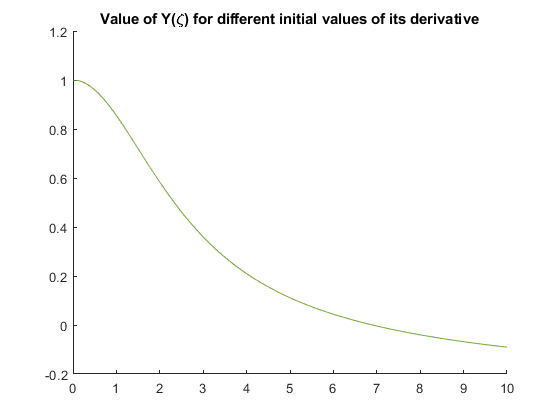
\includegraphics[width=7.3cm]{images/derivades_Y_lluny.png}
    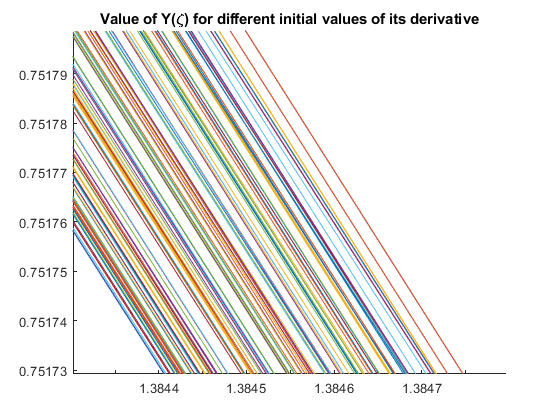
\includegraphics[width=7.3cm]{images/derivades_Y.png}
    \centering
    \caption{Plot of the numerical solutions for different initial values of $\odv{Y}/{\zeta}$}
    \label{fig:derivades}
\end{figure}

The graphic on the left is the view of the total plot and the graphic on the right is taking a deeper look into the curve for different values of the first derivative of $Y$. The value of the derivative of $Y$ at the center of the star should be 0, as the star is in an equilibrium state but to be sure of this assumption we plotted the values from -100 to 100 of the derivative in order to observe if there is a significant change in the curve. As it's observed in the right graphic we must have a very deep look into the values to see a sensible change, so we have considered the value of the derivative to be 0.

\begin{figure}[h]
    \centering
    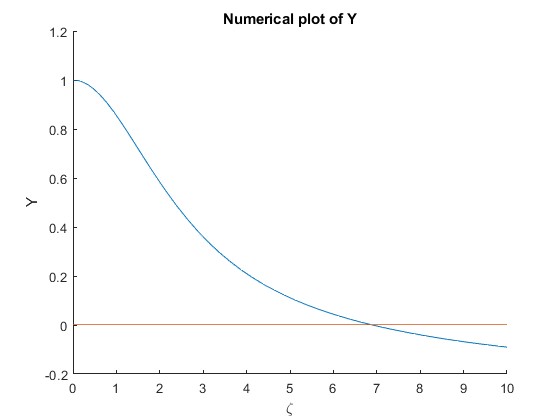
\includegraphics[width=8cm]{images/Y_numerica.png}
    \caption{The numerical plot of $Y$ with respect to $\zeta$, both dimensionless}
    \label{fig:Y_numerica}
\end{figure}

In \autoref{fig:Y_numerica} we can see remarked the straight line $Y=0$. The value of $\zeta$ in which we get $Y=0$ is $\zeta_0$, which is equal to $\frac{R}{a}$, where $R$ is the radius of the star. The understanding of why we find this value for $Y=0$ is because is the place where there is no density, in other words, the boundary of the star.

For the calculus of the limiting mass we will use equation \eqref{eq:massa}, as now we have all the parameters to calculate it. Firstly, we will compute the $Y^3\zeta^2$ for all the numerical values we've got from integrating equation \eqref{eq:aberracio}. When we arrived at this point we fitted the function with a polynomial of order 20 and we used the Matlab function \texttt{polyint} to calculate the primitive of the polynomial and then we used \texttt{polyval} and \texttt{diff} to evaluate the function in its limits. After all of this work we end up getting that the Chandrasekhar limit is $M_c=\qty{1.4360}{\Msun}$.

The fundamental equations we’ve used in order to obtain the Chandrasekhar limit are based on gravitation, for the structure; quantum mechanics, for the momentum of the electrons and special relativity for their energy. If we are dealing with relativistic particles it wouldn’t be more logical to use relativistic quantum mechanics? The answer to this question is that, since we’re dealing with free particles, the expression for the momentum it’s the same regardless of relativity. Another issue related to relativity is the fact that we used non-relativistic fluids mechanics in order to obtain equation \eqref{eq:EDO1}. This treatment is permissible, since, in contrast with electrons, protons and neutrons, which conform the majority of the mass in the star,  do not move at relativistic speeds.

Stars are held by a force equilibrium between the pressure and the gravity. If we compress the star it will raise its pressure, so compressing the star is the way to compensate the gravitational force. Gravity varies as a function proportional to $1/r^2$ so it is difficult to see the existence of an equilibrium for very small radii. In particular, when electrons in the white dwarf become extremely relativistic, as the star compresses itself, the pressure and gravitational forces increase in the same way. There is a point though, where electrons will not have such a significant increase in their speed as the star compresses, as they cannot be faster than light. Thus we observe that there must be a limit in which the star will collapse.

In this derivation of the limit of Chandrasekhar only quantum properties of the electrons and the gravitational force were taken into account. The approaching to the limit implies arbitrarily high densities, so another phenomenon might appear to prevent this to happen. White dwarfs are formed because small stars are incapable of fusing oxygen or carbon. If a white dwarf gets some enough mass to get to the Chandrasekhar limit, then the white dwarf is capable of fusing oxygen and carbon. What we will get at the end is not a white dwarf at the limit. Instead, a thermonuclear explosion that will destroy the star will take place. This explosion is a type I supernova.

\section{Little notes about Neutron stars}

In this section we will discuss a little bit about what a neutron star is in a qualitative way. Neutron stars are celestial bodies which are mainly made of neutrons, as its name can indicate. This neutron stars are the product of the death of a star whose mass is bigger than the Chandrasekhar limit. Those stars, as they were more massive, could fuse elements until iron. Here, the star becomes unstable, as fusion of iron and elements beyond it consume energy rather than generating it, so the nuclear fusion will not take place. Without  nuclear fusion the star will begin to shrink, as there is no force impeding gravity for dominate. This compression will force lead to the creation of a degeneracy pressure, as commented in the white dwarf case, which will not be enough to counteract gravity because we're above the Chandrasekhar limit. 

As before, electrons will begin to move at relativistic speeds and this is favourable for a phenomenon called electron capture takes place. Electron capture is due to weak force and it converts an electron and a proton to a neutron and an electronic neutrino. Thus, the star will begin to have more neutrons in its structure, which have a larger degeneracy pressure. At the beginning of this section we've said that neutron stars are \textit{mostly} made of neutrons. This \textit{mostly} is not put there by coincidence, pure neutron stars do not exist because of $\beta$ decay, in which the neutron decays into an electron, a proton and an electronic antineutrino. The nuclear reactions are summarized below:

\begin{align}
    p+e^-\rightarrow n+\nu_e\\
    n\rightarrow p+e^-+\bar{\nu}_e 
\end{align}

One now can start thinking, why do not all neutrons decay. The answer is again in Pauli exclusion principle. The proton generated must occupy a low energy state. This can happen until a limit where all the low energy states are taken. In this case a new proton would not fit, so the neutron has no other choice to remain as a neutron.

Neutron stars have a limit for their mass, which is the Tolman-Oppenheimer-Volkoff limit. Beyond this limit the star will collapse to a black hole, which has a density that high that even light would not be able to escape its gravitational field.

\section{Conclusion}
In summary, we have found a theoretical expression for the equations that model the structure of a white dwarf. In particular, we approached the deduction of the equation of state from the Fermi gas model in various ways, each time obtaining a similar but different relation. Nonetheless, the use of the most accurate EoS possible is found to be crucial to get reliable results. Finally the numerical resolution of the equations leads to a critical mass limit (that is coherent with accepted bibliography) beyond which a white dwarf is not stable and collapses into a denser body like a neutron star or a black hole.



\newpage
\appendix
\section {Codes used} \label{sec:codes}
These are the Python codes used in \autoref{sec:solvingstructure} and the Matlab code used in \autoref{sec:chandrasekhar}.

\subsection{Code for \autoref{subsec:solvingrel}}
\lstinputlisting[language=Python]{quantum_stars_1.py}
\subsection{Code for \autoref{subsec:solvingnonrel}}
\lstinputlisting[language=Python]{quantum_stars_2.py}
\subsection{Code for \autoref{subsec:solvinggeneral}}
\lstinputlisting[language=Python]{quantum_stars_3.py}

\subsection{Code to calculate the Chandrasekhar limit in \autoref{sec:chandrasekhar}} \label{sec:code_chandrasekhar}
\lstinputlisting[language=Matlab]{matlab_treball_quantum.m}

% \newpage
% \printbibliography[heading=bibintoc]

\end{document}
